%\title{LaTeX Portrait Poster Template}
%%%%%%%%%%%%%%%%%%%%%%%%%%%%%%%%%%%%%%%%%
% a0poster Portrait Poster
% LaTeX Template
% Version 1.0 (22/06/13)
%
% The a0poster class was created by:
% Gerlinde Kettl and Matthias Weiser (tex@kettl.de)
% 
% Adapter by Jens Buysse for Hogeschool Gent
% This template has been downloaded from:
% http://www.LaTeXTemplates.com
%
% License:
% CC BY-NC-SA 3.0 (http://creativecommons.org/licenses/by-nc-sa/3.0/)
%
%%%%%%%%%%%%%%%%%%%%%%%%%%%%%%%%%%%%%%%%%

%----------------------------------------------------------------------------------------
%	PACKAGES AND OTHER DOCUMENT CONFIGURATIONS
%----------------------------------------------------------------------------------------

\documentclass[a0,portrait]{a0poster}

\usepackage{multicol} % This is so we can have multiple columns of text side-by-side
\columnsep=100pt % This is the amount of white space between the columns in the poster
\columnseprule=3pt % This is the thickness of the black line between the columns in the poster

\usepackage[svgnames]{xcolor} % Specify colors by their 'svgnames', for a full list of all colors available see here: http://www.latextemplates.com/svgnames-colors

\usepackage{times} % Use the times font
%\usepackage{palatino} % Uncomment to use the Palatino font

\usepackage{graphicx} % Required for including images
\graphicspath{{figures/}} % Location of the graphics files
\usepackage{booktabs} % Top and bottom rules for table
\usepackage[font=small,labelfont=bf]{caption} % Required for specifying captions to tables and figures
\usepackage{amsfonts, amsmath, amsthm, amssymb} % For math fonts, symbols and environments
\usepackage{wrapfig} % Allows wrapping text around tables and figures
\usepackage[export]{adjustbox}

\begin{document}

%----------------------------------------------------------------------------------------
%	POSTER HEADER 
%----------------------------------------------------------------------------------------

% The header is divided into two boxes:
% The first is 75% wide and houses the title, subtitle, names, university/organization and contact information
% The second is 25% wide and houses a logo for your university/organization or a photo of you
% The widths of these boxes can be easily edited to accommodate your content as you see fit

\begin{minipage}[t]{0.75\linewidth}
\VeryHuge \color{HoGentAccent1} \textbf{Classificatie van afbeeldingen met geautomatiseerde machine learning platformen} \color{Black}\\[2.4cm] % Title
%\Huge\textit{Ondertitel (eventueel)}\\[2.4cm] % Subtitle
\Huge \textbf{Decorte Robbe, dr. Helsens Kenny, ir. Decorte Johan}\\[0.5cm] % Author(s)
\huge Hogeschool Gent, Valentin Vaerwyckweg 1, 9000 Gent\\[0.4cm] % University/organization
\Large \texttt{robbe.decorte@student.hogent.be} \\
\end{minipage}
%
\begin{minipage}[t]{0.25\linewidth}

\includegraphics[width=13cm,right]{figures/HOGENT_Logo_Pos_rgb.png} 

\end{minipage}

\vspace{1cm} % A bit of extra whitespace between the header and poster content

%----------------------------------------------------------------------------------------

\begin{multicols}{2} % This is how many columns your poster will be broken into, a portrait poster is generally split into 2 columns

%----------------------------------------------------------------------------------------
%	ABSTRACT
%----------------------------------------------------------------------------------------

\color{HoGentAccent1} % Navy color for the abstract

\begin{abstract}
De resultaten van dit onderzoek kunnen gebruikt worden om een keuze te maken tussen een open source of cloud platform waar geautomatiseerde \textit{machine learning} gebruikt kan worden. Alsook in welke situaties het bruikbaar is. Het kan een hulp zijn voor bedrijven waar geen \textit{data scientist} of ML-ingenieurs aanwezig zijn. Of waar deze gewoonweg niet genoeg tijd hebben voor de verschillende projecten. Deze technologie tracht \textit{machine learning} toegankelijker te maken door een manier te bieden om vaak voorkomende problemen te automatiseren. Dit werd onderzocht door met AutoKeras en Google Cloud AutoML elk een prototype op te zetten dat voor een simpel maar realistisch classificatieprobleem de categorie van een afbeelding kan voorspellen. Er werden modellen getraind die katten van honden kunnen onderscheiden. Dit document beschrijft een studie naar de achterliggende gebruikte technieken, het verloop en de resultaten van beide prototypes. Er werd gevonden dat de alternatieven elk hun plaats hebben in verschillende fasen van een project. Google Cloud AutoML levert een productie waardig model terwijl AutoKeras kan dienen als hulpmiddel voor een \textit{data scientist} of productie waardig kan zijn mits een extensieve voorbereiding van de data. De evolutie van de platformen zelf betekent enkel goed nieuws voor de toekomst. Mogelijks kan er nog onderzocht worden hoe het opschonen van de data geautomatiseerd kan worden. Dit is een grote stap binnen geautomatiseerde \textit{machine learning} aangezien het een belangrijke factor is om \textit{edge cases} te herkennen.
\end{abstract}
%----------------------------------------------------------------------------------------
%	INTRODUCTION
%----------------------------------------------------------------------------------------

\color{HoGentAccent1} 
\section*{Introductie}
\color{black}
\color{black}

Het informatie tijdperk centraliseert zich momenteel rond data. Bedrijven zien ook de toegevoegde waarde die het kan hebben in hun bedrijfsprocessen, kijk maar naar de grote spelers in de informaticawereld waar het begrip \textit{Big Data} is ontstaan. In zijn ruwe vorm lijkt het op een gigantische hoop waaruit je niks kan leren, maar wanneer men deze gaat structureren zijn er plots allemaal nieuwe toepassingen beschikbaar. 
Eén van deze toepassingen die intensief gebruik maakt van data, is \textit{machine learning}. Hierbij wordt geprobeerd computers zaken aan te leren met behulp van een iteratief proces zonder expliciet geprogrammeerd te zijn voor de taken die ze uitvoeren. Mensen die goed overweg kunnen met de data om zo'n model te maken (Machine Learning Engineers / Data Scientists ...)  zijn vaak moeilijk te vinden. Een werkgever die zo'n probleem aan wilt pakken heeft enkele keuzes, AutoML is een mogelijke optie. Alhoewel het interesseveld ontstaan is in de jaren '50, is het nog maar sinds kort een hot topic, met dank aan de grote hoeveelheid rekenkracht in moderne systemen en doorbraken\footnote{Denk maar aan \textit{open source} initiatieven zoals Tensorflow en Keras.} binnen het onderzoeksveld die de toegangsdrempel verlagen.

Geautomatiseerde \textit{machine learning} platformen trachten een oplossing te bieden voor \textit{development} teams zonder een gespecialiseerde \textit{machine learning} expert. Het platform voert alle stappen van het proces uit en uiteindelijk moeten ze het enkel in hun product integreren. Deze manier van werken verlaagt niet alleen de druk op \textit{machine learning} experten maar het geeft hen ook de mogelijkheid om mee te werken aan uitdagende projecten of zelf onderzoek uit te voeren. Door de technische afhankelijkheid te verlagen kan de technologie sneller / meer gebruikt worden in bestaande projecten. Omdat bedrijven tot nu toe weinig contact hebben met AI en alles wat er toe behoort, zijn de meeste cases vergelijkbaar met elkaar. Zo heb je bijvoorbeeld binaire classificatie problemen, tekst analyse en meer. Waarom zou het dan niet mogelijk zijn om dit te automatiseren? 

Dit onderzoek bekeek hoe laag de werkelijke instapdrempel ligt bij verschillende platformen (open-source en private oplossingen), alsook hoe zo'n model werkt en welke resultaten je bekomt voor een simpel maar realistisch classificatie probleem.

%----------------------------------------------------------------------------------------
%	GEOLOGY
%----------------------------------------------------------------------------------------

\color{Black} % DarkSlateGray color for the rest of the content
\color{HoGentAccent1} 
\section*{Experimenten}
\color{black}


\color{HoGentAccent1} 
\section*{Sectie met figuur}
\color{black}

\begin{center}\vspace{1cm}
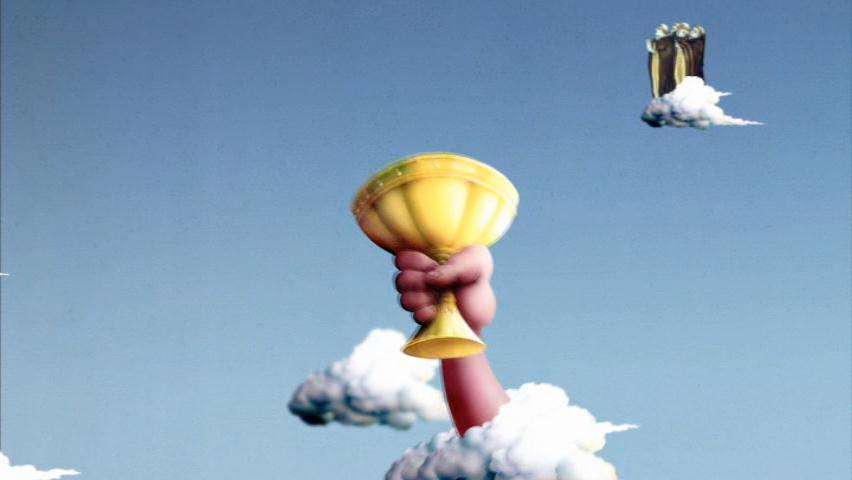
\includegraphics[width=1.0\linewidth]{grail}
\captionof{figure}{\color{HoGentAccent5} He hasn't got shit all over him. The nose? Where'd you get the coconuts? What do you mean? We shall say 'Ni' again to you, if you do not appease us}
\end{center}\vspace{1cm}

%------------------------------------------------



\color{HoGentAccent1} 
\section*{Conclusies}
\color{black}

AutoML is niet goedkoop, zeker op een cloud platform dat snel drie à vierduizend euro per maand kan kosten om operationeel te blijven. Voor AutoKeras zijn de kosten op het eerste zicht beperkt tot verbruikte elektriciteit en \textit{deployment}. Men moet daarbij rekening houden dat elke stap zelf geprogrammeerd moet worden en er toch enige kennis voor nodig is. Het uiteindelijk resultaat wordt dan deels bepaald door de \textit{data preprocessing} die ook handmatig moet gebeuren, deze stap is een belangrijke \textit{trigger} om hoge scores te behalen zoals bij Google Cloud AutoML.

Beide systemen komen de verwachtingen na maar moeten op de juiste plaats ingezet worden. Zo is Google Cloud AutoML een volwaardig \textit{drop in replacement} in bestaande applicaties. Het proces kan niet eenvoudiger zijn en de verschillende manieren om het te integreren zorgen ervoor dat het in meeste situaties past. AutoKeras, in zijn huidige staat, is niet verfijnd genoeg om productie waardig te zijn. De extra moeite om de eerste stappen van het procesmodel te verbeteren kan evengoed verwisseld worden met een ML-ingenieur die het volledige proces uitvoert. Die niche kennis blijft noodzakelijk om te slagen. Anderzijds blijkt het wel een goede \textit{tool} te zijn in de gereedschapskist van ML-ingenieurs.

AutoKeras is sterk gericht op de \textit{core} van het probleem en zo blijven stappen vooraf en achteraf onbeantwoord terwijl die bij de werkwijze van Google Cloud AutoML een aanzienlijke rol hebben. Zo kan een model getraind en \textit{deployed} zijn in een vijftal muisklikken, geen vooraf verwerkte afbeeldingen of andere zaken nodig. Dit terwijl AutoKeras pas gebruikt kan worden nadat de afbeeldingen omgezet zijn naar ruwe data, correct geschaald zijn en grijsfilters of andere optimalisaties toegepast worden. Achteraf is het de verantwoordelijkheid van de gebruiker om het model online te krijgen, wachtrij te optimaliseren en een interface te hebben die kan communiceren met het model.

%----------------------------------------------------------------------------------------
%	FORTHCOMING RESEARCH
%----------------------------------------------------------------------------------------
\color{HoGentAccent1} 
\section*{Toekomstig onderzoek}
\color{black}

De toekomst van geautomatiseerde \textit{machine learning} ziet er alvast goed uit. De verbeteringen tussen versies van AutoKeras vallen op en ook steeds meer cloud platformen bieden een gelijkaardige service aan. Er is een echte \textit{push} aan de gang, van de \textit{community} en de bedrijven, om de toepassingen toegankelijker te maken. Verder onderzoek over dit onderwerp zou zich kunnen richten op individuele stappen van het procesmodel, bijvoorbeeld de \textit{data preprocessing}. De automatisatie ervan is niet vanzelfsprekend omdat dit voor elke dataset anders is.


%----------------------------------------------------------------------------------------

\end{multicols}
\end{document}